\styledchapter{Information Design}

\section{Kamenica and Gentzkow (2012)}

Consider a prosecutor (called the \emph{sender}) and a judge (called the \emph{receiver}), along with a defendant who both the prosecutor and judge believe to be guilty with probability $0.3$.

The prosecutor has utility $1$ if the defendant is convicted and $0$ otherwise.
The judge gets utility $1$ if she makes the correct convict/acquit decision and $0$ otherwise.

The sender chooses two distributions \boxednote{We can think of the sender's choice to be one over requesting a blood test. But we will describe the situation in a general form.}
\[
	\pi(\cdot \mid \text{guilty}), \quad \pi(\cdot \mid \text{innocent})
\] over some set of signals $S$.

If $\left| S \right| = 1$, a single signal comes out regardless of innocence or guilt, so the judge gets no information. Then she acquits.

An opposite approach would be to commit to giving full information: $S \coloneqq  \left\{s_g,s_i\right\}$  with 
\begin{align*}
	\pi(s_g \mid \text{guilty}) &= 1, \quad \pi(s_i \mid \text{guilty}) &&= 0, \\
	\pi(s_g \mid \text{innocent}) &= 0, \quad \pi(s_i \mid \text{innocent}) &&= 1
.\end{align*}
Then the judge convicts with ex-ante probability $0.3$.

Alternatively with $S = \left\{s_g,s_i\right\}$, the sender can distort the signal when the defendant is guilty, putting
\begin{align*}
	\pi(s_g \mid \text{guilty}) &= 1, \quad \pi(s_i \mid \text{guilty}) &&= 0, \\
	\pi(s_g \mid \text{innocent}) &= \alpha, \quad \pi(s_i \mid \text{innocent}) &&= 1-\alpha
.\end{align*}

What is the judge's posterior for the defendant being guilty when the signal received is $s_g$? It is \[
	\P\left[\text{guilty} \mid s_g\right] = \frac{\pi(s_g \mid \text{guilty}) \P\left[\text{guilty}\right] }{\P\left[s_g\right] } = \frac{0.3}{0.3 + 0.7 \cdot \alpha} = \frac{3}{3+7\alpha}
.\] 
\begin{assumption}
	Given the utility assigned, the judge is indifferent between convicting and acquitting when the probability of guilt is $0.5$. We break this tie in favor of conviction.
\end{assumption}

Since having larger $\alpha$ increases the chance of sending $s_g$, we put \[
	\frac{3}{3+7\alpha}  = \frac{1}{2}
,\] while implies the optimal $\alpha$ for the sender is $\alpha^\star = \frac{3}{7}$.

Then the judge convicts with probability \[
	0.3 + 0.7 \cdot \frac{3}{7} = 0.6
.\] 

\section{General Model}

Consider a sender and receiver, finite set of states $\Omega$, and suppose the sender and receiver share a common prior $\mu_0 \in \Delta\left( \Omega \right)$. Assume $\mu_0(\omega) > 0$ for every $\omega \in \Omega$. Let $A$ be a finite set of actions that can be taken by the receiver.

Let $u_S: \Omega \times A \to \R$ and $u_R: \Omega \times A \to \R$.

\begin{definition}[Signal structure]
	A signal structure is a collection of distributions $\left\{\pi(\cdot \mid \omega)\right\}_{\omega \in \Omega}$ where there is a finite set $S$ such that each $\pi(\cdot\mid \omega)$ has support in $S$.
\end{definition}

Given the prior belief $\mu_0$ and the signal structure $\pi$, the receiver forms the posterior $\mu_S$ given each signal $s \in S$ such that \[
	\mu_S(\omega) = \frac{\mu_0(\omega)\pi(s \mid \omega)}{\underbrace{\sum_{\omega'} \mu_0(\omega') \pi(s \mid w')}_{\pi(s)}}
.\] 
The denominator is the probability of receiving signal $s$.

If the receiver has a belief $\mu$, she chooses $\hat{a}(\mu) \in A$ to maximize her expected utility \[
	\hat{a}(\mu) \in \argmax_{a \in A} \sum\limits_{\omega}^{} \mu(\omega) u_R(a,\omega)
.\] 
Assume the receiver breaks ties in favor of the sender.
This induces the expected utility \[
	\hat{u}_S(\mu) = \sum\limits_{\omega}^{} \mu(\omega) u_S(\hat{a}(\mu), w)
.\] 

A signal structure $\left\{\pi\right\}$ induces a distribution $\tau$ over posteriors, i.e.\boxednote{Since $\Omega$ is finite, $\Delta(\Omega)$ can be thought of a simplex, and so $\Delta(\Delta(\Omega))$ is a probability measure on this simplex.} \[
	\tau \in \Delta\left( \Delta (\Omega) \right)
.\] 
$\tau$ has value (the sender's expected utility)\boxednote{We can think of the sender's expected utility as \[
	\int \hat{u}_S(\mu)d\,\tau_\pi(\mu)
.\] } \[
	\int \hat{u}_S(\mu)\,d \tau(\mu)
.\] 

It would be easier to work directly with the distribution of posterior beliefs instead of the signal structure. There is a constraint, though. The sender cannot choose any distribution of posterior beliefs that she wants;\footnote{For example, the prosecutor cannot impose a distribution over posteriors where the judge believes the defendant is guilty with probability $1$.} there must be some signal structure that induces this distribution over posteriors.

\begin{lemma}
	 A necessary condition for a distribution over posteriors to have some signal structure that induces it is that the expectation of the posterior beliefs is the prior. \label{5-20-1}
\end{lemma}
\begin{proof}
	We see that for each $\omega \in \Omega$,
	\begin{align*}
		\sum\limits_{s\in S}^{} \pi(s) \mu_S(\omega)
		&= \sum\limits_{s\in S}^{} \pi(s) \frac{\pi(s \mid \omega) \mu_0(\omega)}{\pi(s)} \\
		&= \sum\limits_{s \in S}^{} \pi(s \mid \omega) \mu_0(\omega) = \mu_0(\omega)
	.\end{align*}
	\texthl{So the expectation of the posteriors something}
\end{proof}

\begin{definition}[Bayes-plausible]
	Given a prior $\mu_0$, $\tau \in \Delta(\Delta(\Omega))$ is Bayes-plausible if \[
		\int \mu\, d \tau(\mu) = \mu_0
	.\] 
\end{definition}

The distribution of posteriors must be Bayes-plausible. In fact, this is the only limitation over the distribution of posteriors. Wow!

\begin{proposition}
	There is a signal structure with value $V^\star$ iff there is a Bayes-plausible distribution over posterior beliefs such that \[
		\int \hat{u}_S(\mu)\, d \tau(\mu) = V^\star
	.\] \label{5-20-2}
\end{proposition}

We first need the following theorem, which we take as given.
\begin{theorem}[Carath\'eodory]
	Suppose $X \subseteq \R^d$ and $y $ is a point in the convex hull of $X$. Then there are $d+1$ points in $X$ such that $y$ is in the convex hull of those points.
\end{theorem}

\propositionproofstyle
\begin{proof}[Proof of Proposition (\ref{5-20-2})]
	($\implies$) was shown in Lemma (\ref{5-20-1}).

	($\impliedby$) Suppose $\tau \in \Delta(\Delta(\Omega))$ is Bayes-plausible and has value $V^\star$. Consider the set $T$ of all pairs $(\hat{u}_S(\mu),\mu)$ for $\mu$ in the support of $\tau$. Note that $T \subseteq \R^{\left| \Omega \right|+ 1}$.

	We have that $(V^\star,\mu_0)$ is in the convex hull of $T$.\boxednote{\texthl{Why?}} By Carath\'eodory's Theorem,\footnote{
	\par
	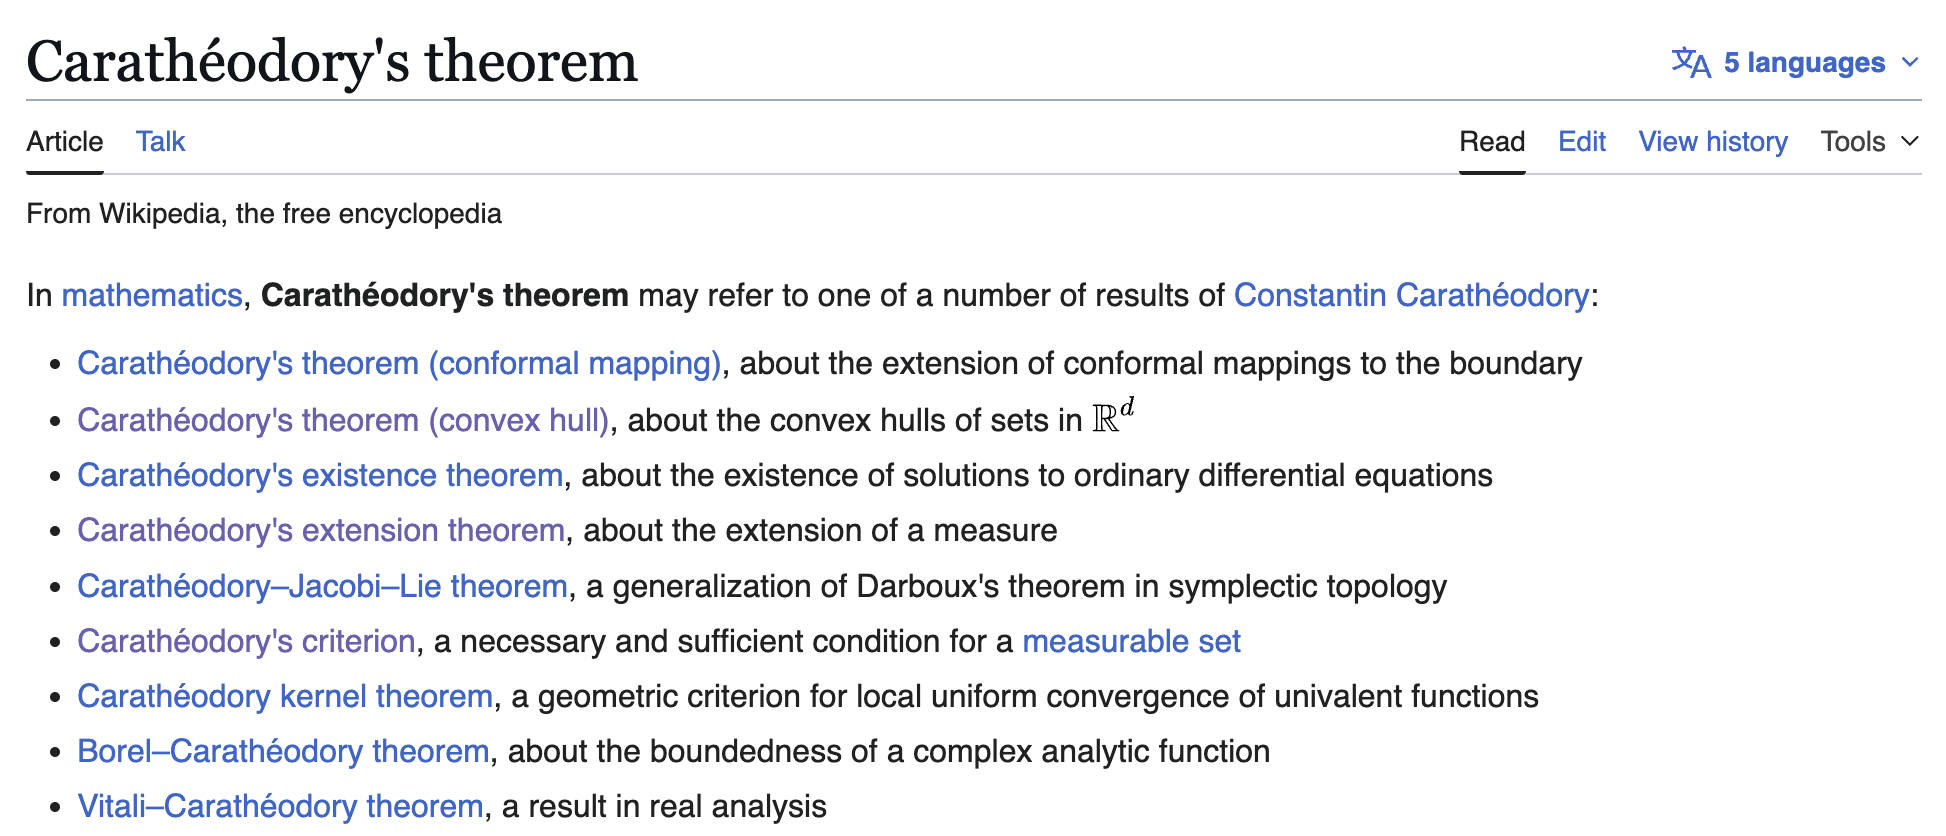
\includegraphics[width=0.38\linewidth]{images/5-20-a}
	\newline
	Pick the right theorem!
	\par
	
	} there is a distribution $\tau^\star$ with finite support $T^\circ$ such that \[
		\sum\limits_{\mu \in T^\circ}^{} \left( \hat{u}_S(\mu),\mu \right)\tau^\star(\mu)  = \left( V^\star, \mu_0 \right)
	.\] 
	We can turn this into a signal structure by setting $S = T^\circ$ and put \[
		\pi(\mu \mid \omega) = \frac{\mu(\omega) \tau^\star(\mu)}{\mu_0(\omega)}
	.\] Now we verify that the belief about $\omega $ given $\mu \in T^\circ$ is \[
		\frac{\pi(\mu \mid \omega) \mu_0(\omega)}{\sum_{\omega'} \mu_0(\omega') \pi(\mu \mid \omega')} = \frac{\mu(\omega) \tau^\star(\mu)}{\sum_{\omega'} \mu_0(\omega') \frac{\mu(\omega') \tau^\star(\mu)}{\mu_0(\omega')}} = \mu(\omega)
	.\] 
\end{proof}

Now let \[
	G \coloneqq  \left\{\left( \hat{u}_S(\mu),\mu \right)\right\}_{\mu \in \Delta(\Omega)}
,\] which is the graph of $\mu$ under $\hat{u}_S$. Let $\operatorname{CO}(G)$ be the convex hull of $G$ and \[
	V(\mu) \coloneqq  \sup \left\{z \mid (z,\mu) \in \text{CO}(G)\right\}
\] be the \emph{concavification} of $\hat{u}$. $V(\mu_0)$ is exactly the optimal utility for the sender.

\begin{center}
	\begin{tikzpicture}[
x=1.05cm,
		y=1.1cm,
		axis/.style={->, thick},
		curve/.style={very thick},
		secant/.style={very thick, blue!70!black},
		guide/.style={densely dashed, black!45},
		gain/.style={densely dashed, very thick, blue!70!black},
		point/.style={circle, fill=black, inner sep=1.35pt},
		valuepoint/.style={circle, fill=blue!70!black, inner sep=1.55pt},
		every node/.style={font=\small}
	]
		\pgfmathsetmacro{\muLeft}{1.3}
		\pgfmathsetmacro{\muRight}{4.7}
		\pgfmathsetmacro{\muZero}{(\muLeft+\muRight)/2}
		\pgfmathsetmacro{\uLeft}{0.32*(\muLeft-\muZero)^2 + 1.15 + 0.15*(\muLeft-\muZero)}
		\pgfmathsetmacro{\uRight}{0.32*(\muRight-\muZero)^2 + 1.15 + 0.15*(\muRight-\muZero)}
		\pgfmathsetmacro{\uZero}{0.32*(\muZero-\muZero)^2 + 1.15 + 0.15*(\muZero-\muZero)}
		\pgfmathsetmacro{\vZero}{(\uLeft+\uRight)/2}

		\coordinate (muprime) at (\muLeft,\uLeft);
		\coordinate (mudprime) at (\muRight,\uRight);
		\coordinate (mugraph) at (\muZero,\uZero);
		\coordinate (muvalue) at (\muZero,\vZero);

		\draw[axis] (-0.15,0) -- (6.15,0) node[right] {$\mu$};
		\draw[axis] (0,-0.1) -- (0,3.75) node[above] {$z$};

		\draw[curve, domain=0.35:\muLeft, samples=90]
			plot (\x,{\uLeft + 0.2*(\x-\muLeft) + 0.27*sin(240*(\x-\muLeft)+180)});
		\draw[curve, domain=\muLeft:5.65, samples=120]
			plot (\x,{0.32*(\x-\muZero)^2 + 1.15 + 0.15*(\x-\muZero)});
		\node[anchor=west, font=\scriptsize] at (5.6,3.75) {$\hat{u}_S(\mu)$};

		\draw[secant] (muprime) -- (mudprime);
		\draw[guide] (\muLeft,0) -- (muprime);
		\draw[guide] (\muRight,0) -- (mudprime);
		\draw[guide] (\muZero,0) -- (muvalue);
		\draw[gain] (mugraph) -- (muvalue);

		\node[point] at (muprime) {};
		\node[anchor=south east, font=\scriptsize] at ($(muprime)+(-0.08,0.22)$) {$\hat{u}_S(\mu')$};
		\node[point] at (mudprime) {};
		\node[anchor=west, font=\scriptsize] at ($(mudprime)+(0.15,-0.03)$) {$\hat{u}_S(\mu'')$};
		\node[point] at (mugraph) {};
		\node[anchor=north west, font=\scriptsize] at ($(mugraph)+(0.15,-0.10)$) {$\hat{u}_S(\mu_0)$};
		\node[valuepoint] at (muvalue) {};
		\node[anchor=south west, font=\scriptsize, blue!70!black] at ($(muvalue)+(0.22,0.2)$) {$V(\mu_0)$};

		\draw (\muLeft,0.05) -- (\muLeft,-0.05) node[below, font=\scriptsize] {$\mu'$};
		\draw (\muZero,0.05) -- (\muZero,-0.05) node[below, font=\scriptsize] {$\mu_0$};
		\draw (\muRight,0.05) -- (\muRight,-0.05) node[below, font=\scriptsize] {$\mu''$};
	\end{tikzpicture}
\end{center}

If $\hat{u}_S$ is concave, then $V = \hat{u}_S$, so there is no benefit to information design. But if it is not concave, there is at least one prior where information design is beneficial.
